\section{Sparse Matrix-Vector Multiplication}
\label{sec:spmv}

Sparse linear algebra libraries and the methods they employ are vitally important in the domain of scientific computing (TODO: why?).  Of particular interest is the sparse matrix-vector product, which solves $y = \bm{A}x$ where $\bm{A}$ is a sparse matrix and the vectors $y$ and $x$ are dense.  Because SpMV usage is often highly repetitive within, e.g., iterative solvers, performance improvements via novel algorithms and the exploitation of modern hardware are areas of ongoing research (TODO: citations).

...why is SpMV difficult? Things like array indirection, varying sparsity patterns, it's memory bound...

As modern hardware introduces higher levels of parallelism and SpMV algorithms become more complex, the likelihood of introducing subtle bugs becomes decidedly higher.  In this section we present a method for reasoning about the structural complexities and verifying the correctness of SpMV algorithms.  We first model an abstract matrix-vector multiplication and subsequently demonstrate that a CSR SpMV algorithm is a valid functional refinement.

\subsection{Abstract Matrix-Vector Multiplication}
\label{sec:mvmabs}

In order to demonstrate that an SpMV algorithm is correct, we must first create a model of matrix-vector multiplication to act as the arbiter of correctness.  The result of the matrix-vector multiplication $y = \bm{A}x$ is a densely populated vector, $y$, in which each value is the dot product of a single row of the matrix $A$ with the vector $x$.  A dot product is simply a sum of products in which each product is of two values located at the same index within two vectors, as shown in ~\figurename~\ref{fig:dp}.

\begin{figure}
\begin{subfigure}[b]{0.5\textwidth}
  \centering
  \begin{tikzpicture}

\matrix (A) [
  matrix of math nodes,
  row sep=.5ex,
  column sep=.5ex,
  left delimiter={[},right delimiter={]},
  nodes={text width=1.5em, text height=1.5ex, text depth=.5ex, align=center}
]
{
  A_{00} & A_{01} & A_{02} \\
  A_{10} & A_{11} & A_{12} \\
  A_{20} & A_{21} & A_{22} \\
};

\node (times) [right=0.75em of A] {$\times$};

\matrix (x) [
  matrix of math nodes,
  left delimiter=\{,
  right delimiter=\},
  row sep=.5ex,
  nodes={text height=1.5ex, text depth=.5ex,}, 
  right=of A
] {
  x_0\\
  x_1\\
  x_2\\
};

\node (eq) [right=1em of x] {$=$};

\matrix (b) [
  matrix of math nodes,
  left delimiter=\{,
  right delimiter=\},
  row sep=.5ex,
  nodes={text height=1.5ex, text depth=.5ex},
  right=1em of eq
] {
  \bm{A_0 \cdot x_0}\\
  A_1 \bm{\cdot} x_1\\
  A_2 \bm{\cdot} x_2\\
};

\end{tikzpicture}
  \caption{}
  \label{fig:mvm}
\end{subfigure}
{\color{lightgray}\rule{0.4\textwidth}{0.1pt}}
\par\bigskip
\begin{subfigure}[b]{0.5\textwidth}
  \centering
  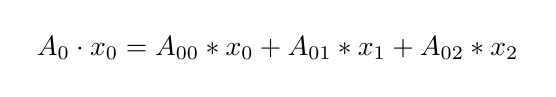
\begin{tikzpicture}
\node (A0x0) {
  $\bm{A_0 \cdot x_0} = A_{00}*x_0 + A_{01}*x_1 + A_{02}*x_2$ 
};
\end{tikzpicture}
  \caption{}
  \label{fig:dp}
\end{subfigure}
{\color{lightgray}\rule{0.4\textwidth}{0.1pt}}
\par\bigskip
\begin{subfigure}[b]{0.5\textwidth}
  \centering
  \begin{myquote}
\Bsig SumProd \Bextends Value \{\\
\TA values: \Bint\\
\TB $\rightarrow$ \Blone (Value-SumProd)\\
\TB $\rightarrow$ (Value-SumProd)\\
\} \{\\
\TA \Ball i: values.\Buniv.\Buniv\ $|$ i $\geq$ 0\\
\}
\end{myquote}
  \caption{}
  \label{fig:dpt}
\end{subfigure}
\caption{(\subref{fig:mvm}) a matrix-vector multiplication, (\subref{fig:dp}) the components of the first dot product in (\subref{fig:mvm}), and (\subref{fig:dpt}) the relational form of the same dot product.}
\end{figure}

Thus far, our matrix and sparse matrix models are capable of representing the structure of the matrix and vectors, as well as the values contained in $\bm{A}$ and $x$.  However, because we wish to model the \emph{structural} behavior of the algorithm, the resulting vector, $y$, cannot simply contain abstract values.  Given a solution generated by a matrix-vector multiplication, we need to be able to verify that the \emph{composition} of a value is correct; that each value present in each dot product originates from the correct location.
%We require a mechanism that allows us to determine the origin of values in the dot product--such a mechanism will allow us to reason about whether or not the dot product is the correct composition of values.  
This is enabled by using the \texttt{SumProd} signature, introduced in Section~\ref{sec:sumprod}, along with the following predicates:
% Building on the \texttt{SumProd} signature, we introduce the following predicates:
(1) to generate dot products, we introduce the \texttt{dotProd} predicate in Section~\ref{sec:dotprod}, (2) to determine the equivalence of dot products we introduce the \texttt{valEqv} predicate in Section~\ref{sec:valeqv}, and (3) to perform an abstract matrix-vector multiplication, we introduce the \texttt{MVM} predicate in Section~\ref{sec:abstractmvm}.
% Additionally, we require some mechanism for equating dot products, allowing us to determine if the solutions generated by differing algorithms are equivalent.  This is achieved using the \texttt{valEqv} predicate introduced in Section~\ref{sec:valeqv}.

\subsubsection{Sum of Products Model}
\label{sec:sumprod}

\begin{figure}
\begin{subfigure}[b]{0.5\textwidth}
  \centering
  \begin{myquote}
\Bsig SumProd \Bextends Value \{\\
\TA values: \Bint\\
\TB $\rightarrow$ \Blone (Value-SumProd)\\
\TB $\rightarrow$ (Value-SumProd)\\
\} \{\\
\TA \Ball i: values.\Buniv.\Buniv\ $|$ i $\geq$ 0\\
\}
\end{myquote}
  \caption{}
  \label{alloy:sumprod}
\end{subfigure}
{\color{lightgray}\rule{0.4\textwidth}{0.1pt}}
\par\bigskip
\begin{subfigure}[b]{0.5\textwidth}
  \centering
  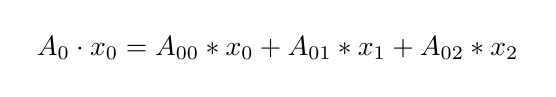
\begin{tikzpicture}
\node (A0x0) {
  $\bm{A_0 \cdot x_0} = A_{00}*x_0 + A_{01}*x_1 + A_{02}*x_2$ 
};
\end{tikzpicture}
  \caption{}
  \label{alloy:dotprod}
\end{subfigure}
{\color{lightgray}\rule{0.4\textwidth}{0.1pt}}
\par\bigskip
\begin{subfigure}[b]{0.5\textwidth}
  \centering
  \begin{myquote}
\Bpred valEqv [x, y: Value] \{\\
\TA (x = y)\\
\TA \Bor (x \Bin SumProd \Band isZero[x] \Band y = Zero)\\
\TA \Bor (y \Bin SumProd \Band isZero[y] \Band x = Zero)\\
\TA \Bor (isZero[x] \Band isZero[y])\\
\TA \Bor (x \Bin SumProd \Band\\
\TB \ y \Bin SumProd \Band\\
\TB \ removeZeros[x] = removeZeros[y])\\
\}
\end{myquote}
  \caption{}
  \label{alloy:valeqv}
\end{subfigure}
\caption{(\subref{alloy:sumprod}) The \texttt{SumProd} signature, representing a summation of products, (\subref{alloy:dotprod}) the \texttt{dotProd} predicate, which assembles a dot product, and (\subref{alloy:valeqv}) the \texttt{valEqv} predicate, which determines if two values are equivalent.}
\end{figure}

The \texttt{SumProd} signature found in ~\figurename~\ref{alloy:sumprod} represents the result of a dot product operation, a sum of products.  Because each dot product evaluates to a single value that must be stored in one of our existing matrix models, the \texttt{SumProd} signature extends \texttt{Value}.  Note that this evaluation is never actually realized, we merely wish to assemble values such that they represent a sum of products.  To do so, \texttt{SumProd} contains a single field, \texttt{values}, that maps unique integers to \texttt{Value} pairs.  We do not allow \texttt{SumProd}s to nest, as we only wish to model dot products of numerical values, not complex numerical expressions, and so \texttt{SumProd} is removed from the set of values that may be stored by using the expression \texttt{(Value-SumProd)}.  Using the \texttt{values} field, the \texttt{SumProd} signature is able to represent a sum of products as a table in which each row contains a product of two values, and the summation is composed of all rows, as shown in \figurename~\ref{fig:dpt}.  Additionally, the integer value associated with each row indicates the index from which the values in that row originate.

\subsubsection{Dot Product Model}
\label{sec:dotprod}

The \texttt{dotProd} predicate found in \figurename~\ref{alloy:dotprod} assembles the dot product of \texttt{row} and \texttt{x} into the \texttt{SumProd} \texttt{b}.  These three arguments warrant an explanation, as their usage may not be immediately clear.

First, the relation \texttt{row} represents a single row from an abstract \texttt{Matrix}.  Recall that a \texttt{Matrix} stores values using an \texttt{Int$\rightarrow$Int$\rightarrow$Value} relation, in which the first and second integer represent the row and column, respectively, in which the corresponding value falls.  Therefore, when we reference all values in a single row, the first integer is removed, leaving us with a relation of the form required by \texttt{row}, which is \texttt{Int$\rightarrow$Value}.  In this relation, the integer represents the column in which the corresponding value falls.

Second, the argument \texttt{x} must be a \texttt{Matrix}, representing the column vector that is being multiplied by the matrix in our matrix-vector multiplication.  Note that we do not enforce certain properties of \texttt{x}, namely that it contain a single column and the same number of rows as the matrix has columns.  It is assumed that these checks are performed in concert with the use of the \texttt{dotProd} predicate.

Finally, the argument \texttt{b} is a \texttt{SumProd}, representing the dot product of \texttt{row} and \texttt{x}.  The set of values contained by this \texttt{SumProd} is fully enumerated within the predicate using the two \texttt{all} statements.  The first one states that for each column index, \texttt{col}, in the current row of the matrix, the \texttt{col}-th value of the dot product summation is equal to the row value at index \texttt{col} times the vector value at (\texttt{col}, 0).  The second states that any integer that is \emph{not} a column index also does not show up in the set of \texttt{SumProd} values.

\subsubsection{Dot Product Equivalence}
\label{sec:valeqv}

When we perform a matrix-vector multiplication, the result is a column vector in which each value is a single \texttt{SumProd}.  So, in order to compare the results of two different matrix-vector multiplication algorithms, we need to be able to determine the equivalence of individual \texttt{SumProd}s.  Additionally, we must be able to determine if a \texttt{SumProd} is equal to \texttt{Zero}, so as not to preclude an algorithm from skipping the assembly of a dot product should it know that a row of the matrix is empty.  Finally, because differing algorithms may be operating on storage structures that contain differing numbers of zeros, we expect the composition of dot products to also contain differing numbers of zeros.  However, we do expect all dot products to contain equivalent sets on nonzero values originating from the same locations.  Therefore, to determine the equivalence of two values, the \texttt{valEqv} predicate, shown in \figurename~\ref{alloy:valeqv}, compares only nonzero values when it encounters a \texttt{SumProd} value.  Note the use of a few helper functions, namely \texttt{isZero} and \texttt{removeZeros}.  The \texttt{isZero} function evaluates to true if the \texttt{SumProd} contains no nonzero values, and the \texttt{removeZeros} function returns the set of nonzero values contained in a \texttt{SumProd}.  These and other helper functions can be found in the supplemental repository~\cite{repository}.

\subsubsection{Matrix-Vector Multiplication Model}
\label{sec:abstractmvm}

\begin{figure}
\begin{myquote}
\Bpred MVM [A, x, b: Matrix] \{\\
% \TA A.rows = b.rows\\
% \TA A.cols = x.rows\\
% \TA x.cols = 1\\
% \TA b.cols = 1\\
% \TA SumProd \Bnot \Bin A.values[\Buniv][\Buniv]\\
% \TA SumProd \Bnot \Bin x.values[\Buniv][\Buniv]\\
\TA \ldots\\
\TA \Ball i: rowInds[A] $|$\\
\TB dotProd[A.values[i], x, b.values[i][0]]\\
\}
\end{myquote}
\caption{The abstract matrix-vector multiplication model.}
\label{alloy:mvmabs}
\end{figure}

Finally, we are able to model a matrix-vector multiplication using the \texttt{MVM} predicate shown in \figurename~\ref{alloy:mvmabs}.  This predicate receives three matrices, \texttt{A}, \texttt{x}, and \texttt{b}.
For brevity, a number of lines have been removed from the \texttt{MVM} predicate.  These lines, which can be found in the supplemental repository~\cite{repository}, simply ensure that \texttt{x} and \texttt{b} each only contain a single column and that the dimensions of all three matrices are able to represent a valid matrix-vector multiplication.
% , the shapes of which are enforced in the first four lines of the predicate.  The \texttt{x} and \texttt{b} matrices are limited to a single column so that they represent column vectors.  The number of rows in \texttt{x} is equal to the number of columns in \texttt{A} so that a matrix-vector multiplication is possible between the two, and the number of rows in \texttt{b} is equal to the number of rows in \texttt{A} so that it can represent the solution to the matrix-vector multiplication.  
Additionally, we enforce that there are no \texttt{SumProd}s present in either \texttt{A} or \texttt{x}.  As mentioned previously, we are only interested in modeling matrix-vector multiplications that consist of simple numerical values.

The \texttt{all} statement in the \texttt{MVM} predicate performs the actual matrix-vector multiplication.  It simply states that the value located at row \texttt{i} in the solution vector \texttt{b} is equal to the dot product of row \texttt{i} of the matrix \texttt{A} with the vector \texttt{x}.

\subsection{CSR Matrix-Vector Multiplication}

In this section we model a CSR matrix-vector multiplication algorithm and demonstrate that it is a valid functional refinement of the matrix-vector multiplication algorithm modeled in Section~\ref{sec:mvmabs}.

Recall that the CSR format contains three arrays.  The arrays \texttt{A} and \texttt{JA} are equal in length and contain values and the column indices at which those values appear, respectively.  The third array, \texttt{IA}, contains integers used to index into \texttt{A} and \texttt{JA}.  Each consecutive pair of indices represents a subset of the \texttt{A} and \texttt{JA} arrays corresponding to a single row of the matrix.  The first pair of indices represents the first row, the second pair represents the second row, and so on.

\LinesNumbered
\begin{algorithm}
\SetStartEndCondition{ }{}{}
\SetKwProg{Fn}{def}{\string:}{}
\SetKwFunction{Range}{range}
\SetKw{KwTo}{in}\SetKwFor{For}{for}{\string:}{}
\SetKwIF{If}{ElseIf}{Else}{if}{:}{elif}{else:}{}
\SetKwFor{While}{while}{:}{fintq}
\newcommand{\forcond}[2]{$#1$ \KwTo\Range{$#2$}}
\SetAlgoNoEnd
\DontPrintSemicolon
\For{\forcond{i}{nrows}}{
  \For{\forcond{j}{\mathrm{IA}[i], \mathrm{IA}[i+1]}} {
    val = A[$j$]\;
    col = JA[$j$]\;
    b[$i$] = b[$i$] + val * x[col]\;
  }
}
\BlankLine
\caption{The CSR MVM algorithm.}
\label{algorithm:csrmvm}
\end{algorithm}
\LinesNotNumbered

Algorithm~\ref{algorithm:csrmvm} performs the matrix-vector multiplication of a CSR matrix with the vector \texttt{x}, resulting in the vector \texttt{b}.  In this algorithm, the inner loop is responsible for iterating over consecutive pairs of indices in the \texttt{IA} array.  Within this inner loop, the current value and column are extracted from the \texttt{A} and \texttt{JA} arrays, and the dot-product is accumulated at the appropriate location.

\begin{figure}
\begin{subfigure}[b]{0.5\textwidth}
  \centering
  \begin{myquote}
\Bpred MVM [C: CSR, x, b: Matrix] \{\\
% \TA C.rows = b.rows\\
% \TA C.cols = x.rows\\
% \TA x.cols = 1\\
% \TA b.cols = 1\\
% \TA SumProd \Bnot \Bin C.A.elems\\
% \TA SumProd \Bnot \Bin x.values[\Buniv][\Buniv]\\
\TA \ldots\\
\TA \Ball i: rowInds[C] $|$\\
\TB \Blet row = getrow[C, i] $|$\\
\TC dotProd[row, x, b.values[i][0]]\\
\}
\end{myquote}
  \caption{}
  \label{alloy:mvmcsr}
\end{subfigure}
{\color{lightgray}\rule{0.4\textwidth}{0.1pt}}
\par\bigskip
\begin{subfigure}[b]{0.5\textwidth}
  \centering
  \begin{myquote}
\Bfun getrow [c: CSR, row: \Bint]: \Bint$\rightarrow$Value \{\\
\TA \Blet cols = rowcols[c, row],\\
\TB vals = rowvals[c, row] $|$ $\sim$cols.vals\\
\}
\end{myquote}
  \caption{}
  \label{alloy:getrow}
\end{subfigure}
{\color{lightgray}\rule{0.4\textwidth}{0.1pt}}
\par\bigskip
\begin{subfigure}[b]{0.5\textwidth}
  \centering
  \begin{myquote}
\Bassert refines \{\\
\TA \Ball C: CSR, M, x, mb, cb: Matrix $|$\\
\TB \ldots\\
\TB alpha[C, M] \Band\\
\TB MVM[C, x, cb] \Band\\
\TB MVM[M, x, mb] \Bimplies matEqv[cb, mb]\\
\}
\end{myquote}
  \caption{}
  \label{alloy:mvmcsrref}
\end{subfigure}
\caption{(\subref{alloy:mvmcsr}) The CSR matrix-vector multiplication model, (\subref{alloy:getrow}) the \texttt{getrow} helper function, which extracts the column$\rightarrow$value pairs of a row in a CSR matrix, and (\subref{alloy:mvmcsrref}) the predicate used to check for refinement.}
\end{figure}

We model Algorithm~\ref{algorithm:csrmvm} in the \texttt{MVM} predicate found in \figurename~\ref{alloy:mvmcsr}.  This predicate shares much in common with the abstract model, still requiring that matrix and vector dimensions are valid for a matrix-vector multiplication.  These lines, just as in the abstract model, have been removed for brevity.

The row loop in the CSR model is modeled in the same way as the row loop in the abstract model, by using an \texttt{all} expression.  Before the inner loop, however, this model uses the \texttt{getrow} helper function to extract the columns and values from the CSR data structure.  This helper function, found in \figurename~\ref{alloy:getrow}, models the array dereferencing found in lines 3 and 4 of Algorithm~\ref{algorithm:csrmvm}.  Additionally, it returns the full set of column$\rightarrow$value pairs for a given row.  This allows us to reuse the \texttt{dotProd} predicate found in \figurename~\ref{alloy:dotprod}.  Note that the \texttt{getrow} function makes use of two additional helper functions, \texttt{rowcols} and \texttt{rowvals}, which extract the sequence of columns and values, respectively, for a given column.  Both can be found in the supplemental repository~\cite{repository}.

Finally, we check that our algorithm correctly performs a matrix-vector multiplication in the \texttt{refines} assertion, found in \figurename~\ref{alloy:mvmcsrref}.  First, the lines that have been removed simply enforce the representation invariant for all of the arguments passed to the predicate.  Next, two matrix-vector multiplications are assembled: $\bm{M} * x = m_b$ and $\bm{C} * x = c_b$.  Additionally, the CSR matrix $\bm{C}$ and abstract matrix $\bm{M}$ are made equivalent using the abstraction function \texttt{alpha}.
% Additionally, the CSR matrix $\bm{C}$ is made to be a refinement of the abstract matrix $\bm{M$} using the abstract function \texttt{alpha}, so that they represent the same matrix.  
The assertion states that if $\bm{M}$ and $\bm{C}$ represent the same matrix and are multiplied by the same vector, $x$, then their respective solution vectors, $m_b$ and $c_b$ are equivalent.

This assertion has been tested for up to 5$\times$5 matrices, and is found to be valid.  Therefore, we can conclude that within scope Algorithm~\ref{algorithm:csrmvm} is correct.